\documentclass[journal,12pt,twocolumn]{IEEEtran}

\usepackage{setspace}
\usepackage{gensymb}

\singlespacing


\usepackage[cmex10]{amsmath}

\usepackage{amsthm}

\usepackage{mathrsfs}
\usepackage{txfonts}
\usepackage{stfloats}
\usepackage{bm}
\usepackage{cite}
\usepackage{cases}
\usepackage{subfig}

\usepackage{longtable}
\usepackage{multirow}

\usepackage{enumitem}
\usepackage{mathtools}
\usepackage{steinmetz}
\usepackage{tikz}
\usepackage{circuitikz}
\usepackage{verbatim}
\usepackage{tfrupee}
\usepackage[breaklinks=true]{hyperref}
\usepackage{graphicx}
\usepackage{tkz-euclide}
\usepackage{float}

\usetikzlibrary{calc,math}
\usepackage{listings}
    \usepackage{color}                                            %%
    \usepackage{array}                                            %%
    \usepackage{longtable}                                        %%
    \usepackage{calc}                                             %%
    \usepackage{multirow}                                         %%
    \usepackage{hhline}                                           %%
    \usepackage{ifthen}                                           %%
    \usepackage{lscape}     
\usepackage{multicol}
\usepackage{chngcntr}

\DeclareMathOperator*{\Res}{Res}

\renewcommand\thesection{\arabic{section}}
\renewcommand\thesubsection{\thesection.\arabic{subsection}}
\renewcommand\thesubsubsection{\thesubsection.\arabic{subsubsection}}

\renewcommand\thesectiondis{\arabic{section}}
\renewcommand\thesubsectiondis{\thesectiondis.\arabic{subsection}}
\renewcommand\thesubsubsectiondis{\thesubsectiondis.\arabic{subsubsection}}


\hyphenation{op-tical net-works semi-conduc-tor}
\def\inputGnumericTable{}                                 %%

\lstset{
%language=C,
frame=single, 
breaklines=true,
columns=fullflexible
}
\makeatletter
\setlength{\@fptop}{0pt}
\makeatother
\begin{document}
\newtheorem{theorem}{Theorem}[section]
\newtheorem{problem}{Problem}
\newtheorem{proposition}{Proposition}[section]
\newtheorem{lemma}{Lemma}[section]
\newtheorem{corollary}[theorem]{Corollary}
\newtheorem{example}{Example}[section]
\newtheorem{definition}[problem]{Definition}

\newcommand{\BEQA}{\begin{eqnarray}}
\newcommand{\EEQA}{\end{eqnarray}}
\newcommand{\define}{\stackrel{\triangle}{=}}
\bibliographystyle{IEEEtran}
\providecommand{\mbf}{\mathbf}
\providecommand{\pr}[1]{\ensuremath{\Pr\left(#1\right)}}
\providecommand{\qfunc}[1]{\ensuremath{Q\left(#1\right)}}
\providecommand{\sbrak}[1]{\ensuremath{{}\left[#1\right]}}
\providecommand{\lsbrak}[1]{\ensuremath{{}\left[#1\right.}}
\providecommand{\rsbrak}[1]{\ensuremath{{}\left.#1\right]}}
\providecommand{\brak}[1]{\ensuremath{\left(#1\right)}}
\providecommand{\lbrak}[1]{\ensuremath{\left(#1\right.}}
\providecommand{\rbrak}[1]{\ensuremath{\left.#1\right)}}
\providecommand{\cbrak}[1]{\ensuremath{\left\{#1\right\}}}
\providecommand{\lcbrak}[1]{\ensuremath{\left\{#1\right.}}
\providecommand{\rcbrak}[1]{\ensuremath{\left.#1\right\}}}
\theoremstyle{remark}
\newtheorem{rem}{Remark}
\newcommand{\sgn}{\mathop{\mathrm{sgn}}}
\providecommand{\abs}[1]{\vert#1\vert}
\providecommand{\res}[1]{\Res\displaylimits_{#1}} 
\providecommand{\norm}[1]{\lVert#1\rVert}
%\providecommand{\norm}[1]{\lVert#1\rVert}
\providecommand{\mtx}[1]{\mathbf{#1}}
\providecommand{\mean}[1]{E[ #1 ]}
\providecommand{\fourier}{\overset{\mathcal{F}}{ \rightleftharpoons}}
%\providecommand{\hilbert}{\overset{\mathcal{H}}{ \rightleftharpoons}}
\providecommand{\system}{\overset{\mathcal{H}}{ \longleftrightarrow}}
	%\newcommand{\solution}[2]{\textbf{Solution:}{#1}}
\newcommand{\solution}{\noindent \textbf{Solution: }}
\newcommand{\cosec}{\,\text{cosec}\,}
\providecommand{\dec}[2]{\ensuremath{\overset{#1}{\underset{#2}{\gtrless}}}}
\newcommand{\myvec}[1]{\ensuremath{\begin{pmatrix}#1\end{pmatrix}}}
\newcommand{\mydet}[1]{\ensuremath{\begin{vmatrix}#1\end{vmatrix}}}
\numberwithin{equation}{subsection}
\makeatletter
\@addtoreset{figure}{problem}
\makeatother
\let\StandardTheFigure\thefigure
\let\vec\mathbf
\renewcommand{\thefigure}{\theproblem}
\def\putbox#1#2#3{\makebox[0in][l]{\makebox[#1][l]{}\raisebox{\baselineskip}[0in][0in]{\raisebox{#2}[0in][0in]{#3}}}}
     \def\rightbox#1{\makebox[0in][r]{#1}}
     \def\centbox#1{\makebox[0in]{#1}}
     \def\topbox#1{\raisebox{-\baselineskip}[0in][0in]{#1}}
     \def\midbox#1{\raisebox{-0.5\baselineskip}[0in][0in]{#1}}
\vspace{3cm}
\title{ASSIGNMENT 5}
\author{Ananthoju Pranav Sai \\ AI20BTECH11004}
\maketitle
\newpage
\bigskip
\renewcommand{\thefigure}{\theenumi}
\renewcommand{\thetable}{\theenumi}
Download all python codes from 
\begin{lstlisting}
https://github.com/Ananthoju-Pranav-Sai/EE3900/blob/main/Assignment-5/codes/Assignment-5.py
\end{lstlisting}
%
and latex-tikz codes from 
%
\begin{lstlisting}
https://github.com/Ananthoju-Pranav-Sai/EE3900/tree/main/Assignment-5/Assignment-5.tex
\end{lstlisting}
%
\section{Quadratic Forms Q.2.62}
Find a point on the curve $y=(x-2)^2$ at which the tangent is parallel to the chord joining the points $\myvec{2\\0}$ and $\myvec{4\\4}$.
\section{Solution}
Equation of the given conic in vector form is 
\begin{align}
    \vec{x}^T\myvec{1 &0\\0 &0}\vec{x}+2\myvec{-2 &\frac{-1}{2}}\vec{x}+4=0 \label{a}
\end{align}
Therefore we have
\begin{align}
    \vec{V} &= \myvec{1 &0\\0 &0}\\
    \vec{u} &= \myvec{-2 \\ \frac{-1}{2}}\\
    f &= 4
\end{align}
Given the tangent is parallel to the chord joining the points $\myvec{2\\0}$ and $\myvec{4\\4}$. So,
\begin{align}
    \vec{m} &= \myvec{4\\4} - \myvec{2\\0}\\
    \vec{m} &= \myvec{2\\4}\\
    \implies \vec{n} &= \myvec{-4\\2}
\end{align}
\begin{lemma}
If $\vec{V}$ is not invertible, given the normal vector $\vec{n}$, the point of contact is given by the matrix equation
\begin{align}
    \myvec{\vec{u}^T+\kappa\vec{n}^T\\\vec{V}}\vec{q} = \myvec{-f\\ \kappa\vec{n}-\vec{q}} 
\end{align} 
where
\begin{align}
    \kappa = \frac{\vec{p_1}^Tu}{\vec{p_1}^Tn}\\
    \vec{V}\vec{p_1}=0
\end{align}
\end{lemma}
So let $\vec{p_1} = \myvec{0\\2}$ as it satisfies $\vec{V}\vec{p_1}=0$ then
\begin{align}
    \kappa &= \frac{\vec{p_1}^Tu}{\vec{p_1}^Tn}\\
    \kappa &= \frac{\myvec{0 &2}\myvec{-2\\\frac{-1}{2}}}{\myvec{0 &2}\myvec{-4\\2}}\\
    \kappa &= \frac{-1}{4}
\end{align}
Now the matrix equation 
\begin{align}
    \myvec{\vec{u}^T+\kappa\vec{n}^T\\\vec{V}}\vec{q} &= \myvec{-f\\ \kappa\vec{n}-\vec{q}}\\
    \myvec{-1 &-1\\1 &0\\0 &0}\vec{q} &= \myvec{-4\\3\\0}\\
    \vec{q} &= \myvec{3\\1}
\end{align}
\begin{figure}[ht]
    \centering
    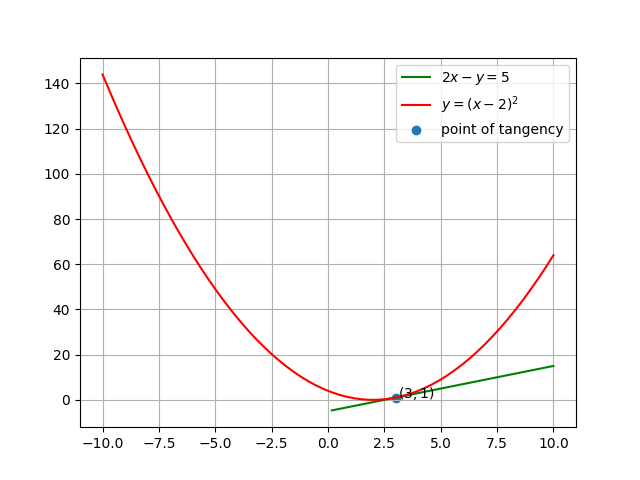
\includegraphics[width=\columnwidth]{plot.png}
    \caption{Plot of the tangent and parabola}
    \label{plot}
\end{figure}
\end{document}
